\chapter{Structural Results}\label{chap:structural-results}


This chapter shall be devoted to looking at some structural results on arithmetic circuits. 
This would help us understand the relevance of shallow circuits in the context of proving lower bounds for arithmetic circuits of arbitrary depth. 

\section{Homogenization}\label{sec:homogenization}

Suppose we have an $n$-variate degree $d$ polynomial computed by an arithmetic circuit $C$. 
How large can the degree of intermediate computations be? 
Potentially, intermediate computations can involve very high degree terms which somehow cancel each other at the root. 
However, the following lemma of Strassen shows that we may assume without much loss of generality that arithmetic circuits never compute polynomials of degree more than the output. 

\begin{definition}[Homogeneous circuits]
A circuit $C$ is said to be \emph{homogeneous} if every gate in the circuit computes a homogeneous polynomial. 
\end{definition}

\begin{lemma}[Homogenization]\label{lem:homogenization}
Let $f$ be an $n$-variate degree $d$ polynomial computed by a circuit $C$ of size $s$. 
Then, for every $0\leq i \leq d$, there is a \emph{homogeneous arithmetic circuit} $C_i'$, of size at most $O(sd^2)$, that computes the degree $i$ homogeneous polynomial in $i$. 
\end{lemma}
\begin{proof}
Assume without loss of generality that the circuit $C$ has all gates with fan-in at most $2$. 
For every gate $g\in C$, define $(d+1)$ gates $g^{(0)},\dots, g^{(d)}$; we shall construct a new circuit $C'$ such that $g^{(i)}$ computes the degree $i$ homogeneous component of the polynomial computed at $g$. 
If $g$ has children $h_1$ and $h_2$, then $C'$ would have the following connections depending on the type of the gate $g$:
\begin{eqnarray*}
\text{$g = h_1 + h_2$}\quad\implies\quad g^{(i)} &=& h_1^{(i)} \spaced{+} h_2^{(i)}\quad\text{for all $i$}\\
\text{$g = h_1 \times h_2$}\quad\implies\quad g^{(i)} &=& \sum_{j=0}^i h_1^{(j)} h_2^{(i-j)}\quad\text{for all $i$}
\end{eqnarray*}
It is easy to check that the size of the circuit $C'$ is at most $O(sd^2)$, and computes all the homogeneous components of $f$. 
\end{proof}

Thus, for arithmetic circuits, we can assume without much loss of generality that we are working with a homogeneous circuit. 

\begin{remark*}
For the class of arithmetic formulas, it is not clear if we can homogeneous without loss of generality. 
If we were to apply the above lemma to an arbitrary arithmetic formula, the resulting object is a homogeneous circuit and not a formula. 
It is unclear if any formula can be homogenized without loss of generality. 
The same is the case even for circuits of a fixed depth, as the above construction doubles the depth of the circuit. 

However, the class of ABPs can also be assumed to be homogeneous without loss of generality. 
We leave this as an exercise. 
\end{remark*}

\begin{exercise}
Prove a similar homogenization lemma for algebraic branching programs. 
\end{exercise}

\section{Interpolation}

A very useful technique in arithmetic complexity is interpolation. Suppose we have a circuit $C$ that computes a polynomial $P(x_1,\ldots, x_n, y)$ and say $\deg_y P = d$. We can interpret the polynomial $P$ as an element of $(\F[\vecx])[y]$, that is we can think of $P$ as a univariate polynomial in $y$ with coefficients being elements of $\F[\vecx]$. 
\[
P(x_1,\ldots, x_n, y) \spaced{=} P_0(x_1,\ldots, x_n) + P_1(x_1,\ldots, x_n) y + \cdots + P_d(x_1,\ldots, x_n) y^d
\]
Given that we can compute $P$ by a circuit $C$, can we also compute one of the coefficients $P_i(x_1,\ldots, x_n)$ by a small circuit? The answer is `Yes' as long as we are working over a large enough field. 

\begin{lemma}[Interpolation]\label{lem:interpolation}
Let $P(x_1,\ldots, x_n, y)$ be a polynomial with $\deg_y P \leq d$. For any set of distinct scalars $\alpha_0, \ldots, \alpha_{d} \in \F$ and for every $i \in \set{0,\ldots, d}$,  each of the coefficient polynomials $P_i(x_1,\ldots, x_n)$ defined above can be expressed as a linear combination of 
\[
\set{P(x_1,\ldots, x_n, \alpha_0), \ldots, P(x_1,\ldots, x_n,\alpha_d)}.
\]
Thus in particular, if $P$ is computed by a size $s$ circuit, then each $P_i$ is computable  by a size $s(d+1)$ circuit. Furthermore, if $P$ is computable by a size $s$ circuit from some class $\mathcal{C}$, then each $P_i$ is computable by a size $s(d+1)$ circuit from the class $\Sigma \mathcal{C}$ (which are circuits with a $+$ gate as a root with $\mathcal{C}$-circuits as its children).
\end{lemma}
\begin{proof}
For this proof we shall use $P(\alpha_i)$ as a short-hand for $P(x_1,\ldots, x_n, \alpha_i)$. Then we have the following matrix identity
\[
\insquare{\begin{array}{cccc}
1 & \alpha_0 & \cdots & \alpha_0^d\\
1 & \alpha_1 & \cdots & \alpha_1^d\\
\vdots & \vdots & \ddots & \vdots\\
1 & \alpha_d & \cdots & \alpha_d^d
\end{array}} \insquare{\begin{array}{c}
P_0\\
P_1 \\
\vdots\\
P_d
\end{array}} \spaced{=}
\insquare{\begin{array}{c}
P(\alpha_0)\\
P(\alpha_1) \\
\vdots\\
P(\alpha_d)
\end{array}}
\]
Observe that the matrix on the left is a Vandermonde matrix, and hence is invertible. This implies that there is some matrix $\inparen{\!\inparen{\beta_{ij}}\!}$, its inverse, such that
\[
\insquare{\begin{array}{c}
P_0\\
P_1 \\
\vdots\\
P_d
\end{array}} \spaced{=}
\insquare{\begin{array}{cccc}
\beta_{00} & \beta_{01} & \cdots & \beta_{0d}\\
\beta_{10} & \beta_{11} & \cdots & \beta_{1d}\\
\vdots & \vdots & \ddots & \vdots\\
\beta_{d0} & \beta_{d1} & \cdots & \beta_{dd}
\end{array}} 
\insquare{\begin{array}{c}
P(\alpha_0)\\
P(\alpha_1) \\
\vdots\\
P(\alpha_d)
\end{array}}
\]
In particular, for each $i \in \set{0,\ldots, d}$,
\[
P_i(x_1,\ldots, x_n) \spaced{=} \beta_0 P(x_1,\ldots, x_n, \alpha_0) + \cdots + \beta_d P(x_1,\ldots, x_n, \alpha_d). 
\]
The size bounds and structure claimed is clear from the above expression.
\end{proof}

The use of interpolation is one of the most important methods when dealing with arithmetic circuits. We would many applications of it later in this article. We just give a couple of concrete applications for now. The first is the computation of partial derivatives in a single variable. We leave this as an easy exercise. 

\begin{exercise}[Computing partial derivatives]
Suppose $P(x_1,\ldots, x_n,y)$ be a polynomial computed by a size $s$ circuit with $\deg_y P \leq d$. Show that for any $i$, the partial derivative
$\frac{\partial^i P}{\partial y^i}$ can be computed by a circuit of size at most $s(d+1)$. 

What about computing mixed partials such as $\frac{\partial^n P}{\partial x_1 \cdots \partial x_n}$?
\end{exercise}

\noindent 
Another important application is the task of computing homogeneous components. 

\subsection{Computing homogeneous components}

Suppose we have a size $s$ circuit $C$ that is computing a polynomial $P$ of degree $d$.
We have already seen in \autoref{lem:homogenization} that we can construct each of the homogeneous components of $P$ by a circuit $C'$ of size at most $sd^2$.
Unfortunately, the construction described in \autoref{sec:homogenization} results in a circuit $C'$ even if we started off with a formula computing $P$.
Furthermore, if $P$ was computable by a constant depth circuit, the construction results in an non-constant depth circuit.
However, the construction in \autoref{lem:homogenization} not just computes the homogeneous components of $P$ but it computes them via a \emph{homogeneous} circuit. If the goal is to just compute the homogeneous components (by a possibly non-homogeneous circuit), one can use interpolation. Furthermore, this method would preserve constant depth as well.

Let us use $\Hom_i(P)$ to denote the homogeneous part of degree $i$, and let $d = \deg(P)$.
\[
P(x_1,\ldots, x_n) \spaced{=} \Hom_0(P) + \cdots + \Hom_d(P)
\]
Let $y$ be a new variable and consider the polynomial $P'(x_1,\ldots, x_n, y) := P(yx_1, \ldots, y x_n)$. Then observe that
\[
P'(x_1,\ldots, x_n) \spaced{=} \Hom_0(P) + y\Hom_1(P) + \cdots + y^d \Hom_d(P).
\]
In other words, each homogeneous component of $P$ is a coefficient of some $y^i$ of $P'(x_1,\ldots, x_n,y)$. Thus, \autoref{lem:interpolation} tells us that we can use a linear combination of evaluations of $P'$ to compute these coefficients. 

We summarize this as a lemma. 

\begin{lemma}[Homogeneous component computations]\label{lem:computing-hom-components}
Let $P(x_1,\ldots, x_n)$ be a polynomial with $\deg P = d$. For any set of distinct scalars $\alpha_0, \ldots, \alpha_{d} \in \F$ and for every $i \in \set{0,\ldots, d}$,  each of the homogeneous components $\Hom_i(P)$ defined above can be expressed as a linear combination of 
\[
\set{P(\alpha_0x_1,\ldots, \alpha_0x_n), \ldots, P(\alpha_dx_1,\ldots, \alpha_dx_n)}.
\]
Thus in particular, if $P$ is computed by a size $s$ circuit, then each $\Hom_i(P)$ is computable  by a size $s(d+1)$ circuit. Furthermore, if $P$ is computable by a size $s$ circuit from some class $\mathcal{C}$, then each $\Hom_i(P)$ is computable by a size $s(d+1)$ circuit from the class $\Sigma \mathcal{C}$ (which are circuits with a $+$ gate as a root with $\mathcal{C}$-circuits as its children).
\end{lemma}

It is important to note that for interpolation, we need to be able to find sufficiently many distinct elements in the base field, and this is possible only if the base field is large enough. 

\begin{exercise}\label{ex:ben-or-trick}
Assume the underlying field is large enough. Find a polynomial sized constant depth circuit that computes $\ESym_d$, the elementary symmetric polynomial of degree $d$, defined as
\[
\ESym_{d}(x_1,\ldots, x_n) \spaced{=} \sum_{1\leq i_1 < i_2 < \cdots < i_d \leq n} x_{i_1} \cdots x_{i_d}.
\]
\end{exercise}

\begin{exercise}
Assume the underlying field is large enough. Find a polynomial sized constant depth circuit that computes \emph{complete homogeneous symmetric polynomial} defined as
\[
\sigma_d(x_1,\ldots, x_n) \spaced{=} \sum_{m \in \set{\text{deg. $d$ monomials}}} m.
\]
\textcolor{gray}{For example, $\sigma_2(x_1,x_2,x_3) = x_1^2 + x_2^2 + x_3^2 + x_1x_2 + x_2x_3 + x_1x_3$.}
\end{exercise}


\section{Depth reduction}

The phenomenon of simulating an arbitrary arithmetic circuit by a \emph{shallow} arithmetic circuit is called \emph{depth reduction}. 
Arithmetic circuits exhibit some remarkable depth reduction results, and we shall go over these in this section. 

\subsection{Depth reduction for arithmetic formulas}

The depth reduction for formulas is quite easy to describe. 
This would also serve as step towards understanding the depth reduction for arithmetic circuits. 
The following depth reduction is due to Brent~\cite{brent74}. 

\begin{lemma}[\cite{brent74}]\label{lem:formula-depth-reduction}
Let $f$ be an $n$-variate degree $d$ polynomial computed by an arithmetic formula $\Phi$ of size $s$. 
Then, $f$ can also be computed by a formula $\Phi'$ of size $s' = \poly(s,n,d)$ and depth $O(\log s)$. 
\end{lemma}
\begin{proof}
Assume without loss of generality that $\Phi$ is a formula of fan-in $2$. 
Starting from the root, walk down to the leaves by always taking the child with a larger sub-tree under it. 
Consider the first node in this path $v$ such that the size of the formula rooted at $v$ is smaller than $\frac{2s}{3}$. 
Let $\Phi_v$ refer to the sub-formula rooted at $v$. 
By the choice of the path from the root, we have
\[
\frac{s}{3} \spaced{\leq} \abs{\Phi_v} \spaced{<} \frac{2s}{3}.
\]
Let $\hat{\Phi}_v$ denote the formula where the sub-formula at $v$ is replaced by a fresh variable $y$. 
Since we are dealing with formulas, $\hat{\Phi}_v$ is a linear polynomial in the variable $y$. 
Hence,
\begin{eqnarray*}
\hat{\Phi}_v(y) & = & A \cdot y \spaced{+} B\\
\text{and,}\quad \Phi & = & A \cdot \Phi_v \spaced{+} B
\end{eqnarray*}
for some polynomials $A$ and $B$. 
But we can compute both $A$ and $B$ from $\hat{\Phi}_v(y)$ as
\begin{eqnarray*}
A & = & \hat{\Phi}_v(1) - \hat{\Phi}_v(0)\\
B & = & \hat{\Phi}_v(0)
\end{eqnarray*}
Thus, 
\[
f \quad = \quad (\hat{\Phi}_v(1) - \hat{\Phi}_v(0))\cdot \Phi_v \spaced{+} \hat{\Phi}_v(0)
\]
All the formulas (i.e. $\hat{\Phi}_v(1)$, $\hat{\Phi}_v(0)$, and $\Phi_v$) in the above equation have size at most $\frac{2s}{3}$. 
Thus, by recursively applying this process on each of these sub-formulas, we obtain
\begin{eqnarray*}
\mathrm{Depth}(s) & = & \mathrm{Depth}(2s/3) \spaced{+} 3\\
\implies \mathrm{Depth}(s) &=& O(\log s)\\
\mathrm{Size}(s) & \leq & 4\cdot \mathrm{Size}(2s/3) \spaced{+} O(1)\\
\implies \mathrm{Size}(s) &=& \poly(s).
\end{eqnarray*}
\end{proof}

\begin{figure}
\begin{center}
\tikzstyle{gate}=[circle,draw=black!50,thick]
\tikzstyle{leaf}=[circle,draw=black!50,fill=black!10,thick]
\tikzstyle{phi}=[rectangle,draw=black!50,fill=black!10,thick]
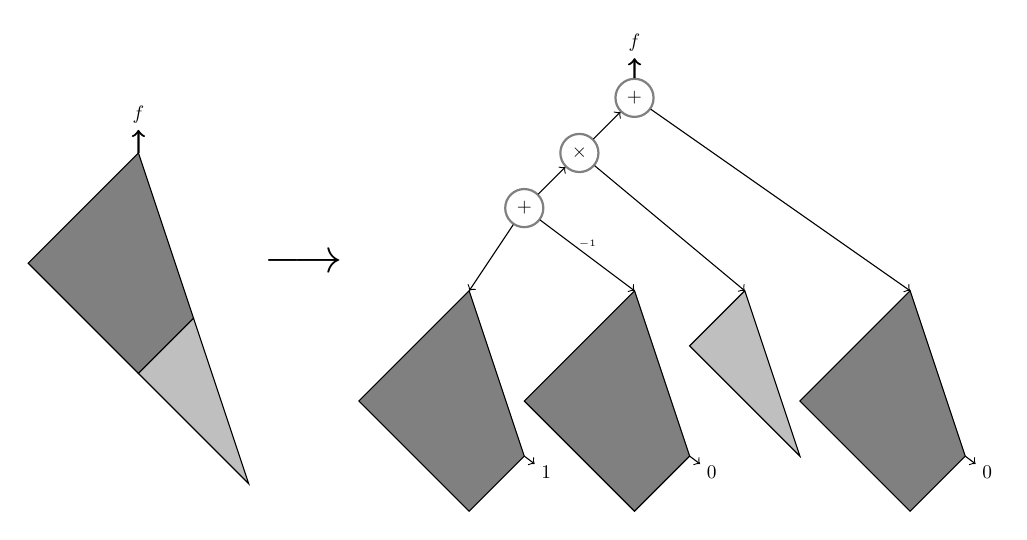
\begin{tikzpicture}[transform shape, scale=0.7]
  \draw[fill=gray] (-10,-2) -- ++(-2,-2) -- ++(2,-2) -- ++(1,1) -- cycle;
  \draw[fill=gray!50] (-9,-5) -- ++(1,-3) -- ++(-2,2) -- cycle;

    \node at (-10,-1.3) {$f$}
    edge[<-,thick] (-10,-2) ;

  
  \node at (-7,-4) {\Huge $\longrightarrow$};
  
  \node (ph) at (-1,0) {$f$};
  \node[gate] (root) at (-1,-1) {$+$}
  edge[thick,->] (ph)
  edge[->] (4,-4.5);
  \node[gate] (m1) at (-2,-2) {$\times$}
  edge[->] (root)
  edge[->] (1,-4.5);
  
  \draw[fill=gray] (4,-4.5) -- ++(-2,-2) -- ++(2,-2) -- ++(1,1) -- cycle;
  \node at  (5.4,-7.8) { $0$}
  edge[<-] (5,-7.5);
  
  \node[gate] (s1) at (-3,-3) {$+$}
  edge[->] (m1)
  edge[->] (-4,-4.5)
  edge[->] node[above] {\tiny $-1$} (-1,-4.5);
  
  \draw[fill=gray!50] (1,-4.5) -- ++(1,-3) -- ++(-2,2) -- cycle;
  
  
  \draw[fill=gray] (-4,-4.5) -- ++(-2,-2) -- ++(2,-2) -- ++(1,1) -- cycle;
  \node at  (-2.6,-7.8) { $1$}
  edge[<-] (-3,-7.5);
  
  \draw[fill=gray] (-1,-4.5) -- ++(-2,-2) -- ++(2,-2) -- ++(1,1) -- cycle;
  \node at  (0.4,-7.8) { $0$}
  edge[<-] (0,-7.5);
\end{tikzpicture}
\end{center}
\caption{Depth reduction for formulas}
\label{fig:formula-depth-red}
\end{figure}

\subsection{Depth reduction for arithmetic circuits}

The key point in the above depth reduction was that for any node $v$, the formulas $\Phi_v$ and $\hat{\Phi}_v(y)$ were disjoint. 
This however is not the case for general arithmetic circuits. 
Thus, it is not clear if we can find a node in the circuit such that the subcircuit under it has size between $s/3$ and $2s/3$. 
However, we do not really need to make the subcircuits have size drop by a constant factor, but any parameter dropping by a constant factor would be fine. 
One parameter that we could work with instead is the \emph{degree}. 


\subsubsection{Applying Brent's reduction with degree}

By \autoref{lem:homogenization}, we may assume that we have a homogeneous circuit $\Phi$ if size $s$ computing a homogeneous $n$-variate polynomial $f$ of degree $d$. 
Using a similar argument as in the proof of \autoref{lem:formula-depth-reduction}, we can find a node $v \in \Phi$ such that $\frac{d}{3} < \deg(v) \leq \frac{2d}{3}$. 
However, we cannot quite write $f$ as $A \cdot \Phi_v + B$ as we are now dealing with a circuit and there could be multiple paths from the root leading to $v$.

Consider the set of all nodes of such intermediate degree as $\mathcal{F}$:
\[
\mathcal{F} = \setdef{v\in \Phi}{\frac{d}{3} < \deg(v)\leq \frac{2d}{3}}
\]
Instead of expressing $f$ using a single $v\in \mathcal{F}$ as in \autoref{lem:formula-depth-reduction}, we shall express $f$ as a function of \emph{all} nodes in $\mathcal{F}$. 

\begin{claim}
If $\mathcal{F} = \inbrace{v_1,\dots, v_s}$, then $f$ may be written as
\begin{equation}\label{eqn:hyafil}
f \spaced{=} \sum_{i,j} A_{ij} \cdot \Phi_{v_i} \Phi_{v_j} \spaced{+} \sum_i B_i \cdot \Phi_{v_i}
\end{equation}
where $\deg(A_{ij}), \deg(B_i) \leq \frac{2d}{3}$ for all $i,j$. 
Moreover, each $A_{ij}$ and $B_i$'s may be computed by an arithmetic circuit of size at most $O(s)$. 
\end{claim}
\begin{proof}
From the circuit $\Phi$, construct the circuit $\Phi'$ that is obtained by removing the incoming edges of every $v_i \in \mathcal{F}$ thereby making these nodes as leaves as well. 
Then, $\Phi'$ computes a polynomial $f'(x_1,\dots x_n, v_1,\dots, v_s)$ satisfying 
\[
f \spaced{=} f'(x_1,\dots, x_n, \Phi_{v_1},\dots, \Phi_{v_s}).
\]
Because of the degree of each $v_i$, we easily obtain that the degree of $f'$ in the $v_i$ variables must be at most $2$, and each coefficient $A_{ij}$ or $B_i$ cannot have degree more than $2d/3$. 
Further, obtaining the $A_{ij}$'s and $B_i$'s from $\Phi'$ is a simple exercise. 
\end{proof}

Since every polynomial appearing in \eqref{eqn:hyafil} is computable by size at most $\poly(s)$ and has degree at most $2d/3$, we may apply induction as earlier. 
Thus,
\begin{eqnarray*}
\mathrm{Depth}(d) & = & \mathrm{Depth}(2d/3) \quad + 2\\
\implies \mathrm{Depth}(d) & = & O(\log d)
\end{eqnarray*}
Unfortunately, the size of the resulting circuit could be as large as $s^{O(\log d)}$. 
This reduction is along the lines of Hyafil~\cite{Hyafil1978}. 

Notice that in this reduction, the final circuit we obtain is in fact an arithmetic formula of size $s^{O(\log d)}$ and depth $O(\log d)$ (assuming that addition gates can have unbounded fan-in; with bounded fan-in addition gates, the depth would be $O(\log d \cdot \log s)$). 
Valiant, Skyum Berkowitz and Rackoff \cite{vsbr83} showed that we can attain a similar depth reduction to $O(\log d)$ depth while keeping the size polynomial. 


\subsubsection{Depth reduction of \cite{vsbr83}}


This section shall be devoted to the proof of the remarkable theorem of Valiant, Skyum, Berkowitz and Rackoff.\footnote{The proof described here follows the structure of a subsequent result \cite{ajmv98}, and not the original proof, although both proofs are quite similar.}


\begin{theorem}[\cite{vsbr83,ajmv98}]\label{thm:vsbr}
  Let $f$ be an $n$-variate degree $d$ polynomial computed by an
  arithmetic circuit $\Phi$ of size $s$. 
Then there is an arithmetic
  circuit $\Phi'$ computing $f$ and has size $s' = \poly(s,n,d)$ and
  depth $O(\log d)$.
\end{theorem}

We may assume without loss of generality that $\Phi$ is a homogeneous
circuit. 
We will also assume that all multiplication gates in $\Phi$
have fan-in at most $2$, and that the degree of the right child of any
multiplication gate is at least as large as the degree of the its left
child. 
Such circuits are known to as \emph{right heavy} circuits. 
For any gate $u$ in $\Phi$, we denote by $[u]$ the polynomial computed at
gate $u$. 
It will also denote a gate label in the new depth reduced
circuit.

We need the following definition of gate quotients.

\begin{definition}\label{defn:gate-quotient}
For any pair of gates $u,v$, the polynomial $[u:v]$ is defined as follows:
\begin{enumerate}
\item If $u$ and $v$ are the same nodes, then $[u:v] = 1$. 
\item If $u$ is a leaf, and $u\neq v$, then $[u:v] = 0$. 
\item If $u = u_1 + u_2$, then $[u:v] = [u_1:v] + [u_2:v]$.
\item If $u = u_1 \times u_2$, then $[u:v] = [u_1] \cdot [u_2 : v]$. \qedhere
\end{enumerate}
\end{definition}

\noindent
It is easy to see that $[u:v]$ is a homogeneous polynomial of degree
$\deg(u) - \deg(v)$. 

\subsection*{Some Intuition}

For an arithmetic formula $\Phi$ with $u$ as root, and any other node
$v$, we can write $\Phi = [u]$ as $A \cdot [v] + B$ for some
polynomials $A$ and $B$. 
We would like to denote $[u:v]$ to denote the
quotient $A$. 
In a circuit things get complicated due to multiple
paths from the $u$ to $v$.

A minimal computation in a circuit is formalized by the notion of a \emph{proof-tree}. 
A proof-tree is a sub-circuit $T$ such that,
\,1. the root is in $T$.
\,2. if a multiplication gate $v$ is in $T$, then so are both its children. 
And,
\,3. if an addition gate $v$ is in $T$, then exactly one child of $v$ is also in $T$.

Every proof-tree computes a monomial, and the polynomial computed by
the circuit is just the sum over all proof-trees. 
The technical issue
in defining the gate quotient stems from the fact that a node $v$
could occur multiple times in a proof-tree, and the number of
occurrences could also vary with different proof-trees. 
To
consistently define the gate quotient, we need to be careful which of
these $v$'s we are referring to. 
We do this by defining the right-most
path in the proof-tree as a canonical path, and replacing the unique
occurrence of $v$ on this canonical path by a leaf labelled $1$ (and
if $v$ does not occur on this path, then this proof-tree does not
contribute to $[u:v]$). 
In fact, it can be seen that
\autoref{defn:gate-quotient} is precisely this notion although
stated algebraically, and this was the perspective used in
\cite{ajmv98}. 
Although it provides more intuition, we
will not use the notion of proof-trees any further to prove
\autoref{thm:vsbr}.

A possible alternate definition is to interpret $u$ as a polynomial in
$v$, and take the first-order partial derivative (as described in
\cite{sy}). 
In the case when $\deg(v) > \deg(u)/2$, this notion
coincides with the above definition of $[u:v]$ (as $v$ cannot occur
more than once in any proof-tree). 
However, some of key properties
(especially \autoref{lem:vsbr-key-lemma} that we shall soon see) are
not true in this setting unless similar degree restrictions are placed
on the pair of nodes. 
While we could reprove \autoref{thm:vsbr} in
this way, we need to be careful about these degree restrictions.

This proof described here can be thought of as a hybrid of
\cite{vsbr83} and \cite{ajmv98}. 
The circuit is built top-down along
the lines of \cite{ajmv98} but using the language of \cite{vsbr83}.


\begin{definition}[Frontier]\label{defn:frontier}
For any parameter $m$, define the \emph{frontier at degree $m$} as
\[
\mathcal{F}_m \quad=\quad \setdef{v}{\deg(v) \geq m\;,\; \deg(v_L), \deg(v_R) < m}
\]
That is, $\mathcal{F}_m$ are the deepest nodes in the circuit that have degree at least $m$. 
\end{definition}

Note that from the above definition, all frontier nodes are
multiplication gates (since we are working with a homogeneous
circuit). 
Also, a frontier forms a maximal anti-chain.

\begin{observation}\label{obs:vsbr-antichain}
  If a node $v$ does not occur in the sub-circuit rooted at $u$, then
  $[u:v] = 0$. 
In particular, if $u, v\in \mathcal{F}_m$ for some $m$, and $u \neq
  v$, then $[u:v]=0$.
\end{observation}

The following is the key lemma for the depth reduction. 

\begin{lemma}\label{lem:vsbr-key-lemma}
Suppose $\Phi$ is a homogeneous, right-heavy circuit. 
Let $m$ be a parameter such that $\deg(u) \geq m$. 
Then,
\begin{equation}\label{eqn:vsbr-for-u}
[u]\spaced{=} \sum_{w\in \mathcal{F}_m} [u:w] \cdot [w]
\end{equation}
Also, if $u,v$ are nodes such that $\deg(u) \geq m > \deg(v)$, then
\begin{equation}\label{eqn:vsbr-for-uv}
[u:v] \spaced{=} \sum_{w\in \mathcal{F}_m} [u:w] [w:v]
\end{equation}
\end{lemma}
\begin{proof}
The proof would be by induction on the depth of $u$.\\

\noindent
1. 
The base case would be when $\deg(u) \geq m$ but all its children have degree less than $m$, that is $u \in \mathcal{F}_m$. 
Such a node $u$ has to be a $\times$ gate. 
Hence,
\begin{eqnarray*}
\sum_{w\in \mathcal{F}_m} [u:w] \cdot [w] &=& [u:u] \cdot [u] \spaced{+}\sum_{\substack{w\in \mathcal{F}_m\\w\neq u}} [u:w] \cdot [w] \spaced{=} [u] \spaced{+} 0\\
\end{eqnarray*}
and
\begin{eqnarray*}
\sum_{w\in \mathcal{F}_m} [u:w] \cdot [w:v] &=& [u:u] \cdot [u:v] \spaced{+}\sum_{\substack{w\in \mathcal{F}_m\\w\neq u}} [u:w] \cdot [w:v] \spaced{=} [u:v] \spaced{+} 0
\end{eqnarray*}
as $[u:w] = 0$ by \autoref{obs:vsbr-antichain}.\\

\noindent
2. 
If $u = u_1 + u_2$,
\begin{eqnarray*}
  [u] &=& [u_1] + [u_2] \\
  &=& \sum_{w\in \mathcal{F}_m} \inparen{[u_1: w]\cdot [w]  + [u_2:w]\cdot [w]}\quad\text{(inductive hypothesis)}\\
  &=& \sum_{w\in \mathcal{F}_m} [u:w] \cdot [w] \quad\text{(\autoref{defn:gate-quotient}.3)}
\end{eqnarray*}
and
\begin{eqnarray*}
  [u:v] &=& [u_1:v] + [u_2:v] \\
  &=& \sum_{w\in \mathcal{F}_m} \inparen{[u_1: w]\cdot [w:v]  + [u_2:w]\cdot [w:v]}\quad\text{(inductive hypothesis)}\\
  &=& \sum_{w\in \mathcal{F}_m} [u:w] \cdot [w:v] \quad\text{(\autoref{defn:gate-quotient}.3)}
\end{eqnarray*}


\noindent
3. 
If $u = u_1 \times u_2$ with $\deg(u_2) \geq m$, 
\begin{eqnarray*}
[u] &=& [u_1] \cdot [u_2]\\
    &=& [u_1] \cdot \inparen{\sum_{w\in \mathcal{F}_m} [u_2:w]\cdot [w]} \quad\text{(inductive hypothesis)}\\
    &=& \sum_{w\in \mathcal{F}_m}([u_1]\cdot [u_2:w]) \cdot [w] = \sum_{w\in \mathcal{F}_m}[u:w] \cdot [w]\quad\text{(\autoref{defn:gate-quotient}.4)}
\end{eqnarray*}
\begin{eqnarray*}
[u:v] &=& [u_1] \cdot [u_2:v]\\
    &=& [u_1] \cdot \inparen{\sum_{w\in \mathcal{F}_m} [u_2:w]\cdot [w:v]} \quad\text{(inductive hypothesis)}\\
    &=& \sum_{w\in \mathcal{F}_m}([u_1]\cdot [u_2:w]) \cdot [w:v] = \sum_{w\in \mathcal{F}_m}[u:w] \cdot [w:v]\quad\text{(\autoref{defn:gate-quotient}.4)}
\end{eqnarray*}

\end{proof}

Now we are ready to write down the depth reduced circuit. 
As mentioned
earlier, the original proof of \cite{vsbr83} follows a bottom-up
approach, but it would be more useful to us to take a top-down
approach (as in \cite{ajmv98}) to obtain some additional structural
properties that we would require.\\

\begin{theorem}[\autoref{thm:vsbr} restated]\label{thm:vsbr-with-structure}
Let $\Phi$ be a homogeneous, right-heavy circuit of size $s$ computing an $n$-variate degree $d$ polynomial. 
Then, there is a circuit $\Phi'$ of size $\poly(s)$ with the following properties:
\begin{enumerate}
\item For every pair of nodes  $u,v\in \Phi$, there are nodes in $\Phi'$ computing $[u]$ and $[u:v]$.
\item For every multiplication gate in $\Phi'$, all its children have at most half its degree. 
\end{enumerate}
\end{theorem}
\begin{proof}
  We shall recursively compute each node $[u]$ and $[u:v]$ from nodes of lower degree. \\

  \noindent
  For any node $u\in \Phi$, let $\mathcal{F}(u) = \mathcal{F}_m$, where
  $m = \deg(u)/2$. 
Thus by \eqref{eqn:vsbr-for-u},
  \begin{eqnarray*}
    [u] & = & \sum_{w\in \mathcal{F}(u)} [u:w] \cdot [w]\\ 
    & = & \sum_{w\in \mathcal{F}(u)} [u:w] \cdot [w_L] \cdot [w_R]
  \end{eqnarray*}
  By our choice of $m$, all the terms on the RHS have degree at most
  $\deg(u)/2$. 
Also, $[u]$ is an addition gate with fan-in $s$ and the
  multiplication gates feeding into it have fan-in $3$.\\
  
  \noindent
  For any pair of nodes $u,v\in \Phi$, let $\mathcal{F}(u,v) =
  \mathcal{F}_m$, where $m = (\deg(u) + \deg(v))/2$. 
By
  \eqref{eqn:vsbr-for-uv},
  \begin{eqnarray*}
    [u:v] & = & \sum_{w\in \mathcal{F}(u,v)} [u:w] \cdot [w:v]\\ 
    & = & \sum_{w\in \mathcal{F}(u,v)} [u:w] \cdot [w_L] \cdot [w_R:v]
  \end{eqnarray*}
  Again by the choice of $m$, the degree of $[u:w]$ and the degree of
  $[w_R:v]$ is at most $(\deg(u) - \deg(v))/2$. 
The degree of $[w_L]$
  however could be as large as $\deg(u) - \deg(v)$. 
Nevertheless, we can
  use the above expansion once more to write it as
  \begin{eqnarray*}
    [u:v] & = & \sum_{w\in \mathcal{F}(u,v)} [u:w] \cdot [w_L] \cdot [w_R:v]\\
    & = & \sum_{w\in \mathcal{F}(u,v)} [u:w] \inparen{\sum_{p \in \mathcal{F}(w_L)} [w_L:p] \cdot [p_L] \cdot [p_R]}\cdot [w_R:v]\\
    & = & \sum_{w\in \mathcal{F}(u,v)}\sum_{p\in \mathcal{F}(w_L)} [u:w] \cdot  [w_L:p] \cdot [p_L] \cdot [p_R]\cdot [w_R:v]
  \end{eqnarray*}
  Now all the terms on the RHS have degree at most $(\deg(u) -
  \deg(v))/2$ as required. 
Also, $[u:v]$ is an addition gate with fan-in
  $s^2$ and the multiplication gates feeding into it have fan-in $5$.\\
  
  Eventually we shall reach a case where $\deg(u)\leq 1$ or $\deg([u:v])
  \leq 1$. 
These are just linear polynomials over $n$ variables and
  shall be explicitly computed in $\Phi'$.

  Starting with the output gate, it is clear how these steps can be
  used to build a depth reduced circuit in a top-down fashion.
\end{proof}

Observe that the proof also shows that all addition gates in $\Phi'$
have fan-in at most $s^2$ and all multiplication gates have fan-in at
most $5$. 
This completes the list of properties we seek from the depth
reduced circuit.


\subsection{Reduction to depth four circuits}

One of the consequence of a depth reduction such as \autoref{thm:vsbr} is that proving lower bounds for general circuits is reduced to the task of proving lower bounds for $O(\log d)$ depth circuits. 

\begin{corollary}\label{cor:vsbr-contra}
If $f$ is an $n$-variate degree $d$ polynomial that requires super-polynomial (in $n$ and $d$) size circuits of $O(\log d)$ depth to compute it, then any general arithmetic circuit computing $f$ must also be of super-polynomial size. 
\end{corollary}

But, optimistically, we would expect that the \emph{right} lower bound must be truly exponential, and not merely super-polynomial. 
Keeping that in mind, a depth reduction even with a slightly super-polynomial blow-up might be useful in this regard. 
This line was first pursued by Agrawal and Vinay \cite{av08}, and the result was subsequently strengthened by Koiran \cite{koiran} and Tavenas~\cite{Tav13}. 

\begin{theorem}[\cite{av08,koiran,Tav13}] \label{thm:av}
Let $f$ be an $n$-variate degree $d$ polynomial computed by a size $s$ arithmetic circuit. 
Then for any $0< t \leq d$, $f$ can be equivalently computed by a homogeneous $\SPSP^{[t]}$ circuit of top fan-in $s^{O(d/t)}$ and size $s^{O(t + d/t)}$. 
\end{theorem}

If we were to optimize the size of the final depth four circuit, then we should choose $t = \sqrt{d}$ to get a $\SPSP^{[t]}$ circuit of size $s^{O(\sqrt{d})}$. 
Note that this implies that if we could prove a lower bound of $n^{\omega(\sqrt{d})}$ for such $\SPSP^{[\sqrt{d}]}$ circuits, then we would have proved a lower bound for general circuits! 
In fact, in the recent past, we have come pretty close to the required threshold and we shall see them in the later chapters. \\

In this section, we shall see a proof of \autoref{thm:av} but this is not the original proof of Tavenas~\cite{Tav13}. 
We shall see an alternate proof by \cite{saptharishivinay14}, which I find more insightful. 

\begin{proofof}{\autoref{thm:av}}
Let $C$ be the $O(\log d)$ depth  circuit computing $f$ obtained from \autoref{thm:vsbr} applied on the size $s$ circuit computing $f$. 
Let $s'$ be the size of $C$. 
If $g$ is a polynomial computed at any intermediate node of $C$, then from the structure of $C$ (~\autoref{thm:vsbr-with-structure}) we have a homogeneous expression
\begin{equation}\label{eqn:vsbr-expansion}
g \spaced{=} \sum_{i=1}^{s'} g_{i1} \cdot g_{i2} \cdot g_{i3} \cdot g_{i4} \cdot g_{i5} 
\end{equation}
where each $g_{ij}$ is computed by a node in $C$ as well, and $\deg(g_{ij}) \leq \deg(g)/2$. 
If we look at \eqref{eqn:vsbr-expansion} for $f$, then the RHS is a $\SPSP^{[d/2]}$ circuit of top fan-in $s'$ computing $f$. 
To obtain a $\SPSP^{[t]}$ circuit eventually, we shall do the following natural process. 
\begin{quote}
  For each summand $g_{i1}\dots g_{ir}$ in the RHS, if the largest degree $g_{ij}$ has degree more than $t$, expand that $g_{ij}$ in-place using \eqref{eqn:vsbr-expansion}. 
  
  Repeat this process until all $g_{ij}$'s on the RHS have degree at most $t$. 
\end{quote}

Note that in each iteration of the above procedure, we increase the top fan-in by a multiplicative factor of $s'$, and what we gain is that some the terms in the RHS would now have smaller degrees. 
If we could show that the in $O(d/t)$  iterations  all terms on the RHS have degree at most $t$, then we would have obtained an $\SPSP^{[t]}$ circuit of top fanin $s'^{O(d/t)}$ computing $f$. \\

To bound the number of iterations, let us count the number of terms of degree more than $t/8$ in each term. 
Note that since we would always maintain homogeneity, the number of terms of degree  $t/8$ or more in any summand  is at most $8d/t$. 
Thus, it suffices to show that each iteration increases the number of terms of degree $t/8$ by at least one. 

Note that in \eqref{eqn:vsbr-expansion}, if $\deg(g) = d'$ then the largest degree term of any summand on the RHS is at least $d'/5$ (since the sum of the degrees of the five terms must add up to $d'$). 
Also, the largest degree term can have degree at most $d'/2$. 
Hence there must be at least $d'/2$ degree contributed by the other four factors in each term. 
This implies that the second largest factor in each summand has degree at least $d'/8$. 
Therefore, as long as we are expanding factors using \eqref{eqn:vsbr-expansion} of degree more than $t/8$, we are guaranteed that each new term has at least one more factor of degree more than $t/8$. 
As argued earlier, we can never have more than $8d/t$ such terms in any summand and this bounds the number of iterations by $8d/t$. 

Thus, when the above procedure stops, we have an $\SPSP^{[t]}$ circuit of top fan-in $s'^{O(8d/t)} = s^{O(d/t)}$. 
Observing that any polynomial of degree $t$ can have at most $n^t$ monomials, we get that the size of the circuit overall is at most $s^{O(t + d/t)}$. 
\end{proofof}

Thus, proving a ``good enough'' top fanin (or size) lower bound for the class of $\SPSP^{[t]}$ circuit would suffice for proving lower bounds for general circuits. 
We would be using this fact quite a lot so we state this explicitly as a corollary. 

\begin{corollary}\label{cor:av}
If $f$ is an $n$-variate degree $d$ polynomial that requires homogeneous $\SPSP^{[t]}$ circuits of top fan-in $n^{\omega(d/t)}$ to compute it, then $f$ requires general arithmetic circuits of size $n^{\omega(1)}$ to compute it. 
\end{corollary}

\begin{exercise}
Define the product-depth of any circuit to be the maximum number of multiplication gates encountered on any root-to-leaf path. 

Show that for any polynomial $n$-variate degree $d$ polynomial $f$ that can be computed by a size $s$ arithmetic circuit, there is a circuit $\Phi'$ of size $s^{O(d^{1/\Delta})}$ and product depth $\Delta$ computing $f$. 
\end{exercise}

\subsection*{Reduction to depth three}

There have been some further depth reductions results. 

\begin{theorem}[\cite{gkks13b}] If $f$ is an $n$-variate degree $d$ polynomial in $\Q[\vecx]$ that can be computed by an arithmetic circuit of size $s$, then it can be equivalently computed by a depth three circuit of size $s^{O(\sqrt{d})}$. 
\end{theorem}

We shall defer this theorem to later in the interest of presenting more insight and intuition. 
They would be better placed after we have seen a few of the recent lower bounds for restricted depth four circuits (but those who are impatient can find it in \autoref{sec:depth-3-red}). 
We now proceed to see some lower bounds. 


\subsection{Depth reduction for formulas, again}

In this section we shall revisit \autoref{thm:av} when it is applied to formulas.
Do the resulting depth four circuits have any additional structure when we start from a homogeneous formula?
The alternate proof of Saptharishi and Vinay~\cite{saptharishivinay14} provides some insight into this. 

We would need the following lemma that was present in the survey of Shpilka and Yehudayoff \cite{sy} and also in the result of Hrube\v{s} and Yehudayoff \cite{HY11a} that we shall see a proof of in \autoref{chap:multilinear} as \autoref{lem:mult-logproduct} and \autoref{lem:hom-logproduct}.


\begin{lemma}[\autoref{lem:hom-logproduct} stated without proof]\label{lem:hom-logproduct-restated}
  Let $\Phi$ be a homogeneous formula of size $s$ computing a polynomial $p$ of degree $d$.
Then $p$ can be written as a sum of $(s+1)$ \emph{log-product} polynomials, that is,
\begin{equation}\label{eqn:dred-formula-logproduct}
p \spaced{=} f_1 + \cdots + f_{r}\quad\quad \text{with $r \leq s+1$}
\end{equation}
where for each $i \in [r]$, we have $f_i = f_{i1} \cdots f_{i\ell}$ satisfying
\begin{itemize}
\item each $f_{ij}$ is homogeneous, and $\sum_j \deg(f_{ij}) = d$,
\item $(1 / 3)^j \cdot d \leq \deg(f_{ij}) \leq (2/ 3)^j \cdot d$,
\item $f_{i\ell} = 1$.
\end{itemize}
In particular, each $f_i$ factors into $\Omega(\log d)$ non-trivial factors of geometrically decreasing degrees. 
\end{lemma}

Furthermore, if $\Phi$ was a multilinear formula to begin with, then so is the expression on the RHS.
And if $\Phi$ was set-multilinear, then so is the expression on the RHS.
In other words, it says that a homogeneous formula has a homogeneous depth-$4$ formula of the form $\Sigma^{[s+1]}\Pi^{[\log d]}\Sigma\Pi^{[2d/3]}$.
We can now describe the mild extension of \autoref{thm:av} applied for homogeneous formulas. 

\begin{theorem}[\autoref{thm:av} for homogeneous formulas]\label{thm:av-formulas}
Let $f$ be a homogeneous $n$-variate degree $d$ polynomial computed by a size $s$ homogeneous formula. 
Then for any $0< t \leq d$, $f$ can be equivalently computed by a homogeneous $\Sigma\Pi^{[a]}\Sigma\Pi^{[t]}$ formula of top fan-in $s^{10(d/t)}$ where 
\[
a \geq \frac{1}{10}\pfrac{d}{t} \log t.
\]
\end{theorem}
What this means is that even though the degree of all polynomials computed by the bottom two levels of the $\SPSP$ circuit have degree bounded by $t$, each summand is a product of much more than $d/t$ factors. Another way to view this is that \autoref{thm:av} gives a $\SPSP$ circuit of size $s^{O(d/t)}$ where the maximum bottom degree and \emph{average bottom degree} are both bounded by $O(t)$. Whereas in the above theorem we have maximum bottom degree bounded by $t$ but \emph{average bottom degree} bounded by $(t / \log t)$. 

\begin{proof}The proof is exactly along the lines of \autoref{thm:av}
  but instead of using the $5$-product expression in \eqref{eqn:vsbr-expansion}, we shall use the log-product expression of \eqref{eqn:dred-formula-logproduct}.
The key point again is that in every such summand, there are two factors of degree at least $d/9$.
Therefore, the proof of \autoref{thm:av} proceeds verbatim and the number of iterations is bounded by $9(d/t)$.
This gives the $\SPSP^{[t]}$ formula of size at most $(s+1)^{9(d/t)} \leq s^{10(d/t)}$.
The only thing left to check is that we do indeed have $\Omega((d\log t) / t)$ non-trivial factors in each summand. We leave this as an exercise with a hint. 
\end{proof}

\begin{exercise} Complete the proof of \autoref{thm:av-formulas} by showing that the number of non-trivial factors in any summand of the resulting $\SPSP^{[t]}$ circuit has $\Omega((d\log t)/t)$ non-trivial factors. 

{\bf Hint:} Show that in \eqref{eqn:dred-formula-logproduct}, in any summand, if we only consider the factors of degree at most $t$, the sum of their degrees is at most $2t$. Use that to say each term must involve $\Omega(d/t)$ expansions via \eqref{eqn:dred-formula-logproduct} thus yielding $\Omega((d\log t)/t)$ factors. 
\end{exercise}

This additional structure may be useful in the quest for proving homogeneous formula lower bounds but at the moment it seems unclear. We shall however see one application of this additional structure later in \autoref{chap:tensorrk}. 

%%% Local Variables: 
%%% mode: latex
%%% TeX-master: "fancymain"
%%% End: 